\documentclass[11pt]{extarticle}
\usepackage[T1]{fontenc}
\usepackage[default]{sourcesanspro}
\usepackage[letterpaper,top=0.8in,bottom=0.8in,left=0.75in,right=0.75in,
  headheight=16pt,headsep=0.22in,footskip=0.4in]{geometry}
\usepackage{tikz}
\usepackage{fancyhdr}
\usepackage{array}
\usepackage{tabularx}
\usepackage{booktabs}
\usepackage{enumitem}
\usepackage{amsmath}
\usepackage{ragged2e}
\usepackage[none]{hyphenat}
\usepackage{titlesec}
\usepackage{needspace}
\usepackage{xltabular}
\usepackage[italic]{mathastext}

\definecolor{cube}{RGB}{176,204,236}
\definecolor{accent}{RGB}{32,78,138}
\definecolor{soft}{RGB}{236,242,250}
\definecolor{mute}{RGB}{95,95,95}

\pagestyle{fancy}
\fancyhf{}
\fancyhead[L]{Week 5 / Tower cities / Adult guide}
\fancyfoot[L]{Bellingham Math Circle / Week 5 / F05-FAC-v4}
\fancyfoot[R]{\thepage}
\renewcommand{\headrulewidth}{0.4pt}
\renewcommand{\footrulewidth}{0pt}

\setlength{\parindent}{0pt}
\setlength{\parskip}{4pt}
\widowpenalty=10000
\clubpenalty=10000
\setlength{\RaggedRightRightskip}{0pt plus 6em}
\setlength{\emergencystretch}{2em}
\RaggedRight
\raggedbottom

\titleformat{\section}{\large\bfseries\color{accent}}{}{0pt}{}
\titlespacing*{\section}{0pt}{10pt}{3pt}
\titleformat{\subsection}{\normalsize\bfseries\color{accent}}{}{0pt}{}
\titlespacing*{\subsection}{0pt}{8pt}{2pt}

% With \raggedbottom every short page costs nothing, so TeX breaks at the most
% negative penalty on the page. Keep headings from attracting breaks, and ask for
% room before a heading without adding a negative penalty.
\makeatletter
\@secpenalty=0
\newcommand{\needlines}[1]{\par\penalty0\begingroup
  \dimen@=#1\relax\dimen@ii=\pagegoal\advance\dimen@ii-\pagetotal
  \ifdim\dimen@>\dimen@ii\ifdim\dimen@ii>\z@\vfil\fi\penalty-\@M\fi\endgroup}
% the last item of a problem stays with the item before it
\newcommand{\lastitem}{\@itempenalty=\@M\item}
\makeatother
\setlist{nosep,leftmargin=1.3em}
\newlist{pbody}{description}{1}
\setlist[pbody]{style=sameline,leftmargin=4.1em,labelwidth=3.7em,labelsep=0.4em,
  align=left,font=\normalfont\itshape\color{mute},itemsep=1.5pt,topsep=1pt,beginpenalty=10000,midpenalty=0}

\newcommand{\core}{\colorbox{accent}{\color{white}\footnotesize\bfseries\,CORE\,}}
\newcommand{\further}{\fcolorbox{accent}{white}{\color{accent}\footnotesize\bfseries\,FURTHER\,}}
\newcommand{\pb}[3]{\par\needlines{4\baselineskip}\addvspace{5pt}\noindent\textbf{Problem #1}\enspace#2\enspace #3\par\nopagebreak[4]}
\newcommand{\hint}[1]{\textbf{(#1)}~}
\newcommand{\tsub}[1]{\needlines{9\baselineskip}\subsection{#1}}

% a small side view of a row of towers: \tw{1,3,2}
\newcommand{\tw}[1]{\begin{tikzpicture}[baseline=0pt,x=1mm,y=1mm]
  \foreach \h [count=\i from 0] in {#1}{
    \foreach \k in {1,...,\h}{\draw[fill=cube,line width=0.25pt] (\i*2.5,\k*1.4-1.4) rectangle ++(2.0,1.4);}
    \draw[line width=0.5pt] (\i*2.5-0.25,0) -- ++(2.5,0);}
\end{tikzpicture}}

% generated by check.py from the computed solutions; do not edit
\newcommand{\MthreeSola}{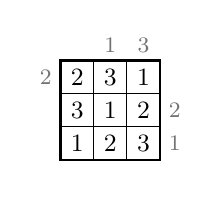
\begin{tikzpicture}[x=0.42cm,y=0.42cm]
\draw[line width=0.4pt] (1,0) -- (1,3);
\draw[line width=0.4pt] (0,1) -- (3,1);
\draw[line width=0.4pt] (2,0) -- (2,3);
\draw[line width=0.4pt] (0,2) -- (3,2);
\draw[line width=1pt] (0,0) rectangle (3,3);
\node at (0.5,2.5) {\small 2};
\node at (1.5,2.5) {\small 3};
\node at (2.5,2.5) {\small 1};
\node at (0.5,1.5) {\small 3};
\node at (1.5,1.5) {\small 1};
\node at (2.5,1.5) {\small 2};
\node at (0.5,0.5) {\small 1};
\node at (1.5,0.5) {\small 2};
\node at (2.5,0.5) {\small 3};
\node[text=black!55] at (1.5,3.45) {\footnotesize 1};
\node[text=black!55] at (2.5,3.45) {\footnotesize 3};
\node[text=black!55] at (-0.45,2.5) {\footnotesize 2};
\node[text=black!55] at (3.45,1.5) {\footnotesize 2};
\node[text=black!55] at (3.45,0.5) {\footnotesize 1};
\path (-1,-1) rectangle (4,4);
\end{tikzpicture}}
\newcommand{\MthreeSolb}{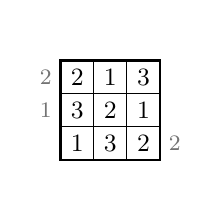
\begin{tikzpicture}[x=0.42cm,y=0.42cm]
\draw[line width=0.4pt] (1,0) -- (1,3);
\draw[line width=0.4pt] (0,1) -- (3,1);
\draw[line width=0.4pt] (2,0) -- (2,3);
\draw[line width=0.4pt] (0,2) -- (3,2);
\draw[line width=1pt] (0,0) rectangle (3,3);
\node at (0.5,2.5) {\small 2};
\node at (1.5,2.5) {\small 1};
\node at (2.5,2.5) {\small 3};
\node at (0.5,1.5) {\small 3};
\node at (1.5,1.5) {\small 2};
\node at (2.5,1.5) {\small 1};
\node at (0.5,0.5) {\small 1};
\node at (1.5,0.5) {\small 3};
\node at (2.5,0.5) {\small 2};
\node[text=black!55] at (-0.45,2.5) {\footnotesize 2};
\node[text=black!55] at (-0.45,1.5) {\footnotesize 1};
\node[text=black!55] at (3.45,0.5) {\footnotesize 2};
\path (-1,-1) rectangle (4,4);
\end{tikzpicture}}
\newcommand{\MthreeSold}{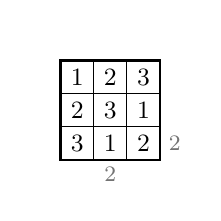
\begin{tikzpicture}[x=0.42cm,y=0.42cm]
\draw[line width=0.4pt] (1,0) -- (1,3);
\draw[line width=0.4pt] (0,1) -- (3,1);
\draw[line width=0.4pt] (2,0) -- (2,3);
\draw[line width=0.4pt] (0,2) -- (3,2);
\draw[line width=1pt] (0,0) rectangle (3,3);
\node at (0.5,2.5) {\small 1};
\node at (1.5,2.5) {\small 2};
\node at (2.5,2.5) {\small 3};
\node at (0.5,1.5) {\small 2};
\node at (1.5,1.5) {\small 3};
\node at (2.5,1.5) {\small 1};
\node at (0.5,0.5) {\small 3};
\node at (1.5,0.5) {\small 1};
\node at (2.5,0.5) {\small 2};
\node[text=black!55] at (3.45,0.5) {\footnotesize 2};
\node[text=black!55] at (1.5,-0.45) {\footnotesize 2};
\path (-1,-1) rectangle (4,4);
\end{tikzpicture}}
\newcommand{\MfourSola}{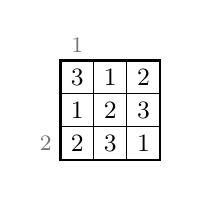
\begin{tikzpicture}[x=0.42cm,y=0.42cm]
\draw[line width=0.4pt] (1,0) -- (1,3);
\draw[line width=0.4pt] (0,1) -- (3,1);
\draw[line width=0.4pt] (2,0) -- (2,3);
\draw[line width=0.4pt] (0,2) -- (3,2);
\draw[line width=1pt] (0,0) rectangle (3,3);
\node at (0.5,2.5) {\small 3};
\node at (1.5,2.5) {\small 1};
\node at (2.5,2.5) {\small 2};
\node at (0.5,1.5) {\small 1};
\node at (1.5,1.5) {\small 2};
\node at (2.5,1.5) {\small 3};
\node at (0.5,0.5) {\small 2};
\node at (1.5,0.5) {\small 3};
\node at (2.5,0.5) {\small 1};
\node[text=black!55] at (0.5,3.45) {\footnotesize 1};
\node[text=black!55] at (-0.45,0.5) {\footnotesize 2};
\path (-1,-1) rectangle (4,4);
\end{tikzpicture}}
\newcommand{\MfourSolb}{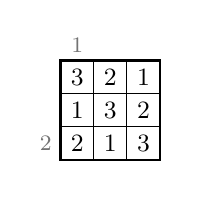
\begin{tikzpicture}[x=0.42cm,y=0.42cm]
\draw[line width=0.4pt] (1,0) -- (1,3);
\draw[line width=0.4pt] (0,1) -- (3,1);
\draw[line width=0.4pt] (2,0) -- (2,3);
\draw[line width=0.4pt] (0,2) -- (3,2);
\draw[line width=1pt] (0,0) rectangle (3,3);
\node at (0.5,2.5) {\small 3};
\node at (1.5,2.5) {\small 2};
\node at (2.5,2.5) {\small 1};
\node at (0.5,1.5) {\small 1};
\node at (1.5,1.5) {\small 3};
\node at (2.5,1.5) {\small 2};
\node at (0.5,0.5) {\small 2};
\node at (1.5,0.5) {\small 1};
\node at (2.5,0.5) {\small 3};
\node[text=black!55] at (0.5,3.45) {\footnotesize 1};
\node[text=black!55] at (-0.45,0.5) {\footnotesize 2};
\path (-1,-1) rectangle (4,4);
\end{tikzpicture}}
\newcommand{\MfourSolc}{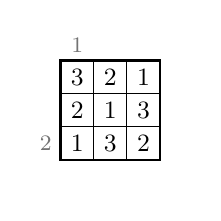
\begin{tikzpicture}[x=0.42cm,y=0.42cm]
\draw[line width=0.4pt] (1,0) -- (1,3);
\draw[line width=0.4pt] (0,1) -- (3,1);
\draw[line width=0.4pt] (2,0) -- (2,3);
\draw[line width=0.4pt] (0,2) -- (3,2);
\draw[line width=1pt] (0,0) rectangle (3,3);
\node at (0.5,2.5) {\small 3};
\node at (1.5,2.5) {\small 2};
\node at (2.5,2.5) {\small 1};
\node at (0.5,1.5) {\small 2};
\node at (1.5,1.5) {\small 1};
\node at (2.5,1.5) {\small 3};
\node at (0.5,0.5) {\small 1};
\node at (1.5,0.5) {\small 3};
\node at (2.5,0.5) {\small 2};
\node[text=black!55] at (0.5,3.45) {\footnotesize 1};
\node[text=black!55] at (-0.45,0.5) {\footnotesize 2};
\path (-1,-1) rectangle (4,4);
\end{tikzpicture}}
\newcommand{\UthreeSola}{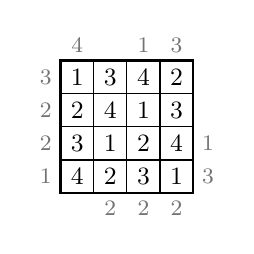
\begin{tikzpicture}[x=0.42cm,y=0.42cm]
\draw[line width=0.4pt] (1,0) -- (1,4);
\draw[line width=0.4pt] (0,1) -- (4,1);
\draw[line width=0.4pt] (2,0) -- (2,4);
\draw[line width=0.4pt] (0,2) -- (4,2);
\draw[line width=0.4pt] (3,0) -- (3,4);
\draw[line width=0.4pt] (0,3) -- (4,3);
\draw[line width=1pt] (0,0) rectangle (4,4);
\node at (0.5,3.5) {\small 1};
\node at (1.5,3.5) {\small 3};
\node at (2.5,3.5) {\small 4};
\node at (3.5,3.5) {\small 2};
\node at (0.5,2.5) {\small 2};
\node at (1.5,2.5) {\small 4};
\node at (2.5,2.5) {\small 1};
\node at (3.5,2.5) {\small 3};
\node at (0.5,1.5) {\small 3};
\node at (1.5,1.5) {\small 1};
\node at (2.5,1.5) {\small 2};
\node at (3.5,1.5) {\small 4};
\node at (0.5,0.5) {\small 4};
\node at (1.5,0.5) {\small 2};
\node at (2.5,0.5) {\small 3};
\node at (3.5,0.5) {\small 1};
\node[text=black!55] at (0.5,4.45) {\footnotesize 4};
\node[text=black!55] at (2.5,4.45) {\footnotesize 1};
\node[text=black!55] at (3.5,4.45) {\footnotesize 3};
\node[text=black!55] at (-0.45,3.5) {\footnotesize 3};
\node[text=black!55] at (-0.45,2.5) {\footnotesize 2};
\node[text=black!55] at (-0.45,1.5) {\footnotesize 2};
\node[text=black!55] at (-0.45,0.5) {\footnotesize 1};
\node[text=black!55] at (4.45,1.5) {\footnotesize 1};
\node[text=black!55] at (4.45,0.5) {\footnotesize 3};
\node[text=black!55] at (1.5,-0.45) {\footnotesize 2};
\node[text=black!55] at (2.5,-0.45) {\footnotesize 2};
\node[text=black!55] at (3.5,-0.45) {\footnotesize 2};
\path (-1,-1) rectangle (5,5);
\end{tikzpicture}}
\newcommand{\UthreeSolb}{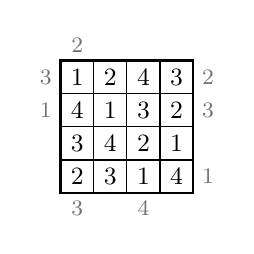
\begin{tikzpicture}[x=0.42cm,y=0.42cm]
\draw[line width=0.4pt] (1,0) -- (1,4);
\draw[line width=0.4pt] (0,1) -- (4,1);
\draw[line width=0.4pt] (2,0) -- (2,4);
\draw[line width=0.4pt] (0,2) -- (4,2);
\draw[line width=0.4pt] (3,0) -- (3,4);
\draw[line width=0.4pt] (0,3) -- (4,3);
\draw[line width=1pt] (0,0) rectangle (4,4);
\node at (0.5,3.5) {\small 1};
\node at (1.5,3.5) {\small 2};
\node at (2.5,3.5) {\small 4};
\node at (3.5,3.5) {\small 3};
\node at (0.5,2.5) {\small 4};
\node at (1.5,2.5) {\small 1};
\node at (2.5,2.5) {\small 3};
\node at (3.5,2.5) {\small 2};
\node at (0.5,1.5) {\small 3};
\node at (1.5,1.5) {\small 4};
\node at (2.5,1.5) {\small 2};
\node at (3.5,1.5) {\small 1};
\node at (0.5,0.5) {\small 2};
\node at (1.5,0.5) {\small 3};
\node at (2.5,0.5) {\small 1};
\node at (3.5,0.5) {\small 4};
\node[text=black!55] at (0.5,4.45) {\footnotesize 2};
\node[text=black!55] at (-0.45,3.5) {\footnotesize 3};
\node[text=black!55] at (-0.45,2.5) {\footnotesize 1};
\node[text=black!55] at (4.45,3.5) {\footnotesize 2};
\node[text=black!55] at (4.45,2.5) {\footnotesize 3};
\node[text=black!55] at (4.45,0.5) {\footnotesize 1};
\node[text=black!55] at (0.5,-0.45) {\footnotesize 3};
\node[text=black!55] at (2.5,-0.45) {\footnotesize 4};
\path (-1,-1) rectangle (5,5);
\end{tikzpicture}}
\newcommand{\UthreeSolc}{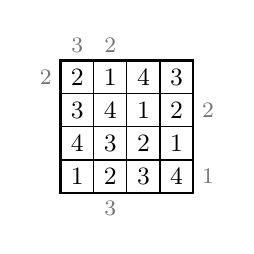
\begin{tikzpicture}[x=0.42cm,y=0.42cm]
\draw[line width=0.4pt] (1,0) -- (1,4);
\draw[line width=0.4pt] (0,1) -- (4,1);
\draw[line width=0.4pt] (2,0) -- (2,4);
\draw[line width=0.4pt] (0,2) -- (4,2);
\draw[line width=0.4pt] (3,0) -- (3,4);
\draw[line width=0.4pt] (0,3) -- (4,3);
\draw[line width=1pt] (0,0) rectangle (4,4);
\node at (0.5,3.5) {\small 2};
\node at (1.5,3.5) {\small 1};
\node at (2.5,3.5) {\small 4};
\node at (3.5,3.5) {\small 3};
\node at (0.5,2.5) {\small 3};
\node at (1.5,2.5) {\small 4};
\node at (2.5,2.5) {\small 1};
\node at (3.5,2.5) {\small 2};
\node at (0.5,1.5) {\small 4};
\node at (1.5,1.5) {\small 3};
\node at (2.5,1.5) {\small 2};
\node at (3.5,1.5) {\small 1};
\node at (0.5,0.5) {\small 1};
\node at (1.5,0.5) {\small 2};
\node at (2.5,0.5) {\small 3};
\node at (3.5,0.5) {\small 4};
\node[text=black!55] at (0.5,4.45) {\footnotesize 3};
\node[text=black!55] at (1.5,4.45) {\footnotesize 2};
\node[text=black!55] at (-0.45,3.5) {\footnotesize 2};
\node[text=black!55] at (4.45,2.5) {\footnotesize 2};
\node[text=black!55] at (4.45,0.5) {\footnotesize 1};
\node[text=black!55] at (1.5,-0.45) {\footnotesize 3};
\path (-1,-1) rectangle (5,5);
\end{tikzpicture}}
\newcommand{\UthreeSold}{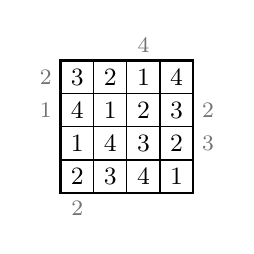
\begin{tikzpicture}[x=0.42cm,y=0.42cm]
\draw[line width=0.4pt] (1,0) -- (1,4);
\draw[line width=0.4pt] (0,1) -- (4,1);
\draw[line width=0.4pt] (2,0) -- (2,4);
\draw[line width=0.4pt] (0,2) -- (4,2);
\draw[line width=0.4pt] (3,0) -- (3,4);
\draw[line width=0.4pt] (0,3) -- (4,3);
\draw[line width=1pt] (0,0) rectangle (4,4);
\node at (0.5,3.5) {\small 3};
\node at (1.5,3.5) {\small 2};
\node at (2.5,3.5) {\small 1};
\node at (3.5,3.5) {\small 4};
\node at (0.5,2.5) {\small 4};
\node at (1.5,2.5) {\small 1};
\node at (2.5,2.5) {\small 2};
\node at (3.5,2.5) {\small 3};
\node at (0.5,1.5) {\small 1};
\node at (1.5,1.5) {\small 4};
\node at (2.5,1.5) {\small 3};
\node at (3.5,1.5) {\small 2};
\node at (0.5,0.5) {\small 2};
\node at (1.5,0.5) {\small 3};
\node at (2.5,0.5) {\small 4};
\node at (3.5,0.5) {\small 1};
\node[text=black!55] at (2.5,4.45) {\footnotesize 4};
\node[text=black!55] at (-0.45,3.5) {\footnotesize 2};
\node[text=black!55] at (-0.45,2.5) {\footnotesize 1};
\node[text=black!55] at (4.45,2.5) {\footnotesize 2};
\node[text=black!55] at (4.45,1.5) {\footnotesize 3};
\node[text=black!55] at (0.5,-0.45) {\footnotesize 2};
\path (-1,-1) rectangle (5,5);
\end{tikzpicture}}
\newcommand{\UthreeSole}{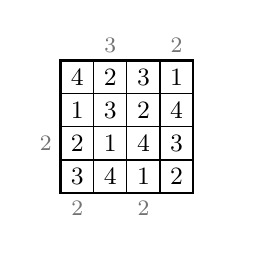
\begin{tikzpicture}[x=0.42cm,y=0.42cm]
\draw[line width=0.4pt] (1,0) -- (1,4);
\draw[line width=0.4pt] (0,1) -- (4,1);
\draw[line width=0.4pt] (2,0) -- (2,4);
\draw[line width=0.4pt] (0,2) -- (4,2);
\draw[line width=0.4pt] (3,0) -- (3,4);
\draw[line width=0.4pt] (0,3) -- (4,3);
\draw[line width=1pt] (0,0) rectangle (4,4);
\node at (0.5,3.5) {\small 4};
\node at (1.5,3.5) {\small 2};
\node at (2.5,3.5) {\small 3};
\node at (3.5,3.5) {\small 1};
\node at (0.5,2.5) {\small 1};
\node at (1.5,2.5) {\small 3};
\node at (2.5,2.5) {\small 2};
\node at (3.5,2.5) {\small 4};
\node at (0.5,1.5) {\small 2};
\node at (1.5,1.5) {\small 1};
\node at (2.5,1.5) {\small 4};
\node at (3.5,1.5) {\small 3};
\node at (0.5,0.5) {\small 3};
\node at (1.5,0.5) {\small 4};
\node at (2.5,0.5) {\small 1};
\node at (3.5,0.5) {\small 2};
\node[text=black!55] at (1.5,4.45) {\footnotesize 3};
\node[text=black!55] at (3.5,4.45) {\footnotesize 2};
\node[text=black!55] at (-0.45,1.5) {\footnotesize 2};
\node[text=black!55] at (0.5,-0.45) {\footnotesize 2};
\node[text=black!55] at (2.5,-0.45) {\footnotesize 2};
\path (-1,-1) rectangle (5,5);
\end{tikzpicture}}
\newcommand{\UthreeSolf}{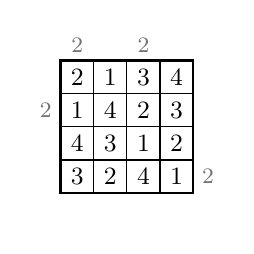
\begin{tikzpicture}[x=0.42cm,y=0.42cm]
\draw[line width=0.4pt] (1,0) -- (1,4);
\draw[line width=0.4pt] (0,1) -- (4,1);
\draw[line width=0.4pt] (2,0) -- (2,4);
\draw[line width=0.4pt] (0,2) -- (4,2);
\draw[line width=0.4pt] (3,0) -- (3,4);
\draw[line width=0.4pt] (0,3) -- (4,3);
\draw[line width=1pt] (0,0) rectangle (4,4);
\node at (0.5,3.5) {\small 2};
\node at (1.5,3.5) {\small 1};
\node at (2.5,3.5) {\small 3};
\node at (3.5,3.5) {\small 4};
\node at (0.5,2.5) {\small 1};
\node at (1.5,2.5) {\small 4};
\node at (2.5,2.5) {\small 2};
\node at (3.5,2.5) {\small 3};
\node at (0.5,1.5) {\small 4};
\node at (1.5,1.5) {\small 3};
\node at (2.5,1.5) {\small 1};
\node at (3.5,1.5) {\small 2};
\node at (0.5,0.5) {\small 3};
\node at (1.5,0.5) {\small 2};
\node at (2.5,0.5) {\small 4};
\node at (3.5,0.5) {\small 1};
\node[text=black!55] at (0.5,4.45) {\footnotesize 2};
\node[text=black!55] at (2.5,4.45) {\footnotesize 2};
\node[text=black!55] at (-0.45,2.5) {\footnotesize 2};
\node[text=black!55] at (4.45,0.5) {\footnotesize 2};
\path (-1,-1) rectangle (5,5);
\end{tikzpicture}}
\newcommand{\UfourSola}{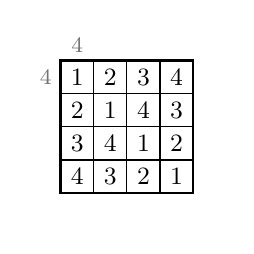
\begin{tikzpicture}[x=0.42cm,y=0.42cm]
\draw[line width=0.4pt] (1,0) -- (1,4);
\draw[line width=0.4pt] (0,1) -- (4,1);
\draw[line width=0.4pt] (2,0) -- (2,4);
\draw[line width=0.4pt] (0,2) -- (4,2);
\draw[line width=0.4pt] (3,0) -- (3,4);
\draw[line width=0.4pt] (0,3) -- (4,3);
\draw[line width=1pt] (0,0) rectangle (4,4);
\node at (0.5,3.5) {\small 1};
\node at (1.5,3.5) {\small 2};
\node at (2.5,3.5) {\small 3};
\node at (3.5,3.5) {\small 4};
\node at (0.5,2.5) {\small 2};
\node at (1.5,2.5) {\small 1};
\node at (2.5,2.5) {\small 4};
\node at (3.5,2.5) {\small 3};
\node at (0.5,1.5) {\small 3};
\node at (1.5,1.5) {\small 4};
\node at (2.5,1.5) {\small 1};
\node at (3.5,1.5) {\small 2};
\node at (0.5,0.5) {\small 4};
\node at (1.5,0.5) {\small 3};
\node at (2.5,0.5) {\small 2};
\node at (3.5,0.5) {\small 1};
\node[text=black!55] at (0.5,4.45) {\footnotesize 4};
\node[text=black!55] at (-0.45,3.5) {\footnotesize 4};
\path (-1,-1) rectangle (5,5);
\end{tikzpicture}}
\newcommand{\UfourSolb}{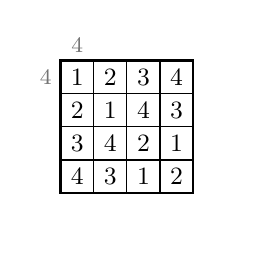
\begin{tikzpicture}[x=0.42cm,y=0.42cm]
\draw[line width=0.4pt] (1,0) -- (1,4);
\draw[line width=0.4pt] (0,1) -- (4,1);
\draw[line width=0.4pt] (2,0) -- (2,4);
\draw[line width=0.4pt] (0,2) -- (4,2);
\draw[line width=0.4pt] (3,0) -- (3,4);
\draw[line width=0.4pt] (0,3) -- (4,3);
\draw[line width=1pt] (0,0) rectangle (4,4);
\node at (0.5,3.5) {\small 1};
\node at (1.5,3.5) {\small 2};
\node at (2.5,3.5) {\small 3};
\node at (3.5,3.5) {\small 4};
\node at (0.5,2.5) {\small 2};
\node at (1.5,2.5) {\small 1};
\node at (2.5,2.5) {\small 4};
\node at (3.5,2.5) {\small 3};
\node at (0.5,1.5) {\small 3};
\node at (1.5,1.5) {\small 4};
\node at (2.5,1.5) {\small 2};
\node at (3.5,1.5) {\small 1};
\node at (0.5,0.5) {\small 4};
\node at (1.5,0.5) {\small 3};
\node at (2.5,0.5) {\small 1};
\node at (3.5,0.5) {\small 2};
\node[text=black!55] at (0.5,4.45) {\footnotesize 4};
\node[text=black!55] at (-0.45,3.5) {\footnotesize 4};
\path (-1,-1) rectangle (5,5);
\end{tikzpicture}}
\newcommand{\UfourSolc}{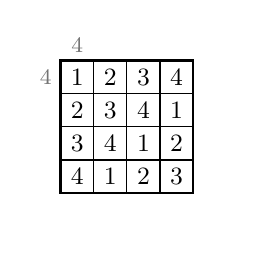
\begin{tikzpicture}[x=0.42cm,y=0.42cm]
\draw[line width=0.4pt] (1,0) -- (1,4);
\draw[line width=0.4pt] (0,1) -- (4,1);
\draw[line width=0.4pt] (2,0) -- (2,4);
\draw[line width=0.4pt] (0,2) -- (4,2);
\draw[line width=0.4pt] (3,0) -- (3,4);
\draw[line width=0.4pt] (0,3) -- (4,3);
\draw[line width=1pt] (0,0) rectangle (4,4);
\node at (0.5,3.5) {\small 1};
\node at (1.5,3.5) {\small 2};
\node at (2.5,3.5) {\small 3};
\node at (3.5,3.5) {\small 4};
\node at (0.5,2.5) {\small 2};
\node at (1.5,2.5) {\small 3};
\node at (2.5,2.5) {\small 4};
\node at (3.5,2.5) {\small 1};
\node at (0.5,1.5) {\small 3};
\node at (1.5,1.5) {\small 4};
\node at (2.5,1.5) {\small 1};
\node at (3.5,1.5) {\small 2};
\node at (0.5,0.5) {\small 4};
\node at (1.5,0.5) {\small 1};
\node at (2.5,0.5) {\small 2};
\node at (3.5,0.5) {\small 3};
\node[text=black!55] at (0.5,4.45) {\footnotesize 4};
\node[text=black!55] at (-0.45,3.5) {\footnotesize 4};
\path (-1,-1) rectangle (5,5);
\end{tikzpicture}}
\newcommand{\UfourSold}{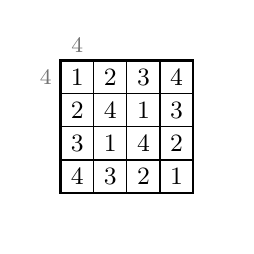
\begin{tikzpicture}[x=0.42cm,y=0.42cm]
\draw[line width=0.4pt] (1,0) -- (1,4);
\draw[line width=0.4pt] (0,1) -- (4,1);
\draw[line width=0.4pt] (2,0) -- (2,4);
\draw[line width=0.4pt] (0,2) -- (4,2);
\draw[line width=0.4pt] (3,0) -- (3,4);
\draw[line width=0.4pt] (0,3) -- (4,3);
\draw[line width=1pt] (0,0) rectangle (4,4);
\node at (0.5,3.5) {\small 1};
\node at (1.5,3.5) {\small 2};
\node at (2.5,3.5) {\small 3};
\node at (3.5,3.5) {\small 4};
\node at (0.5,2.5) {\small 2};
\node at (1.5,2.5) {\small 4};
\node at (2.5,2.5) {\small 1};
\node at (3.5,2.5) {\small 3};
\node at (0.5,1.5) {\small 3};
\node at (1.5,1.5) {\small 1};
\node at (2.5,1.5) {\small 4};
\node at (3.5,1.5) {\small 2};
\node at (0.5,0.5) {\small 4};
\node at (1.5,0.5) {\small 3};
\node at (2.5,0.5) {\small 2};
\node at (3.5,0.5) {\small 1};
\node[text=black!55] at (0.5,4.45) {\footnotesize 4};
\node[text=black!55] at (-0.45,3.5) {\footnotesize 4};
\path (-1,-1) rectangle (5,5);
\end{tikzpicture}}
\newcommand{\Msample}{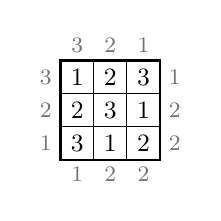
\begin{tikzpicture}[x=0.42cm,y=0.42cm]
\draw[line width=0.4pt] (1,0) -- (1,3);
\draw[line width=0.4pt] (0,1) -- (3,1);
\draw[line width=0.4pt] (2,0) -- (2,3);
\draw[line width=0.4pt] (0,2) -- (3,2);
\draw[line width=1pt] (0,0) rectangle (3,3);
\node at (0.5,2.5) {\small 1};
\node at (1.5,2.5) {\small 2};
\node at (2.5,2.5) {\small 3};
\node at (0.5,1.5) {\small 2};
\node at (1.5,1.5) {\small 3};
\node at (2.5,1.5) {\small 1};
\node at (0.5,0.5) {\small 3};
\node at (1.5,0.5) {\small 1};
\node at (2.5,0.5) {\small 2};
\node[text=black!55] at (0.5,3.45) {\footnotesize 3};
\node[text=black!55] at (0.5,-0.45) {\footnotesize 1};
\node[text=black!55] at (1.5,3.45) {\footnotesize 2};
\node[text=black!55] at (1.5,-0.45) {\footnotesize 2};
\node[text=black!55] at (2.5,3.45) {\footnotesize 1};
\node[text=black!55] at (2.5,-0.45) {\footnotesize 2};
\node[text=black!55] at (-0.45,2.5) {\footnotesize 3};
\node[text=black!55] at (3.45,2.5) {\footnotesize 1};
\node[text=black!55] at (-0.45,1.5) {\footnotesize 2};
\node[text=black!55] at (3.45,1.5) {\footnotesize 2};
\node[text=black!55] at (-0.45,0.5) {\footnotesize 1};
\node[text=black!55] at (3.45,0.5) {\footnotesize 2};
\path (-1,-1) rectangle (4,4);
\end{tikzpicture}}
\newcommand{\UsixSol}{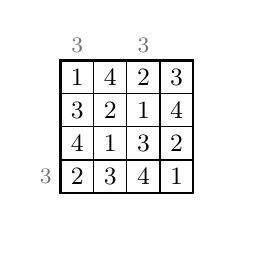
\begin{tikzpicture}[x=0.42cm,y=0.42cm]
\draw[line width=0.4pt] (1,0) -- (1,4);
\draw[line width=0.4pt] (0,1) -- (4,1);
\draw[line width=0.4pt] (2,0) -- (2,4);
\draw[line width=0.4pt] (0,2) -- (4,2);
\draw[line width=0.4pt] (3,0) -- (3,4);
\draw[line width=0.4pt] (0,3) -- (4,3);
\draw[line width=1pt] (0,0) rectangle (4,4);
\node at (0.5,3.5) {\small 1};
\node at (1.5,3.5) {\small 4};
\node at (2.5,3.5) {\small 2};
\node at (3.5,3.5) {\small 3};
\node at (0.5,2.5) {\small 3};
\node at (1.5,2.5) {\small 2};
\node at (2.5,2.5) {\small 1};
\node at (3.5,2.5) {\small 4};
\node at (0.5,1.5) {\small 4};
\node at (1.5,1.5) {\small 1};
\node at (2.5,1.5) {\small 3};
\node at (3.5,1.5) {\small 2};
\node at (0.5,0.5) {\small 2};
\node at (1.5,0.5) {\small 3};
\node at (2.5,0.5) {\small 4};
\node at (3.5,0.5) {\small 1};
\node[text=black!55] at (0.5,4.45) {\footnotesize 3};
\node[text=black!55] at (2.5,4.45) {\footnotesize 3};
\node[text=black!55] at (-0.45,0.5) {\footnotesize 3};
\path (-1,-1) rectangle (5,5);
\end{tikzpicture}}
\newcommand{\UnineA}{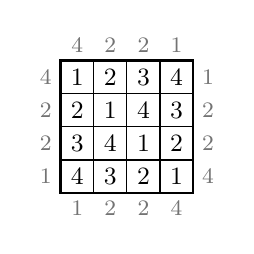
\begin{tikzpicture}[x=0.42cm,y=0.42cm]
\draw[line width=0.4pt] (1,0) -- (1,4);
\draw[line width=0.4pt] (0,1) -- (4,1);
\draw[line width=0.4pt] (2,0) -- (2,4);
\draw[line width=0.4pt] (0,2) -- (4,2);
\draw[line width=0.4pt] (3,0) -- (3,4);
\draw[line width=0.4pt] (0,3) -- (4,3);
\draw[line width=1pt] (0,0) rectangle (4,4);
\node at (0.5,3.5) {\small 1};
\node at (1.5,3.5) {\small 2};
\node at (2.5,3.5) {\small 3};
\node at (3.5,3.5) {\small 4};
\node at (0.5,2.5) {\small 2};
\node at (1.5,2.5) {\small 1};
\node at (2.5,2.5) {\small 4};
\node at (3.5,2.5) {\small 3};
\node at (0.5,1.5) {\small 3};
\node at (1.5,1.5) {\small 4};
\node at (2.5,1.5) {\small 1};
\node at (3.5,1.5) {\small 2};
\node at (0.5,0.5) {\small 4};
\node at (1.5,0.5) {\small 3};
\node at (2.5,0.5) {\small 2};
\node at (3.5,0.5) {\small 1};
\node[text=black!55] at (0.5,4.45) {\footnotesize 4};
\node[text=black!55] at (0.5,-0.45) {\footnotesize 1};
\node[text=black!55] at (1.5,4.45) {\footnotesize 2};
\node[text=black!55] at (1.5,-0.45) {\footnotesize 2};
\node[text=black!55] at (2.5,4.45) {\footnotesize 2};
\node[text=black!55] at (2.5,-0.45) {\footnotesize 2};
\node[text=black!55] at (3.5,4.45) {\footnotesize 1};
\node[text=black!55] at (3.5,-0.45) {\footnotesize 4};
\node[text=black!55] at (-0.45,3.5) {\footnotesize 4};
\node[text=black!55] at (4.45,3.5) {\footnotesize 1};
\node[text=black!55] at (-0.45,2.5) {\footnotesize 2};
\node[text=black!55] at (4.45,2.5) {\footnotesize 2};
\node[text=black!55] at (-0.45,1.5) {\footnotesize 2};
\node[text=black!55] at (4.45,1.5) {\footnotesize 2};
\node[text=black!55] at (-0.45,0.5) {\footnotesize 1};
\node[text=black!55] at (4.45,0.5) {\footnotesize 4};
\path (-1,-1) rectangle (5,5);
\end{tikzpicture}}
\newcommand{\UnineB}{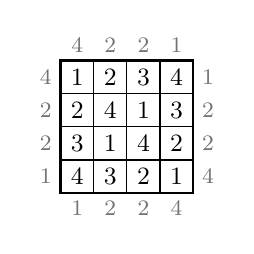
\begin{tikzpicture}[x=0.42cm,y=0.42cm]
\draw[line width=0.4pt] (1,0) -- (1,4);
\draw[line width=0.4pt] (0,1) -- (4,1);
\draw[line width=0.4pt] (2,0) -- (2,4);
\draw[line width=0.4pt] (0,2) -- (4,2);
\draw[line width=0.4pt] (3,0) -- (3,4);
\draw[line width=0.4pt] (0,3) -- (4,3);
\draw[line width=1pt] (0,0) rectangle (4,4);
\node at (0.5,3.5) {\small 1};
\node at (1.5,3.5) {\small 2};
\node at (2.5,3.5) {\small 3};
\node at (3.5,3.5) {\small 4};
\node at (0.5,2.5) {\small 2};
\node at (1.5,2.5) {\small 4};
\node at (2.5,2.5) {\small 1};
\node at (3.5,2.5) {\small 3};
\node at (0.5,1.5) {\small 3};
\node at (1.5,1.5) {\small 1};
\node at (2.5,1.5) {\small 4};
\node at (3.5,1.5) {\small 2};
\node at (0.5,0.5) {\small 4};
\node at (1.5,0.5) {\small 3};
\node at (2.5,0.5) {\small 2};
\node at (3.5,0.5) {\small 1};
\node[text=black!55] at (0.5,4.45) {\footnotesize 4};
\node[text=black!55] at (0.5,-0.45) {\footnotesize 1};
\node[text=black!55] at (1.5,4.45) {\footnotesize 2};
\node[text=black!55] at (1.5,-0.45) {\footnotesize 2};
\node[text=black!55] at (2.5,4.45) {\footnotesize 2};
\node[text=black!55] at (2.5,-0.45) {\footnotesize 2};
\node[text=black!55] at (3.5,4.45) {\footnotesize 1};
\node[text=black!55] at (3.5,-0.45) {\footnotesize 4};
\node[text=black!55] at (-0.45,3.5) {\footnotesize 4};
\node[text=black!55] at (4.45,3.5) {\footnotesize 1};
\node[text=black!55] at (-0.45,2.5) {\footnotesize 2};
\node[text=black!55] at (4.45,2.5) {\footnotesize 2};
\node[text=black!55] at (-0.45,1.5) {\footnotesize 2};
\node[text=black!55] at (4.45,1.5) {\footnotesize 2};
\node[text=black!55] at (-0.45,0.5) {\footnotesize 1};
\node[text=black!55] at (4.45,0.5) {\footnotesize 4};
\path (-1,-1) rectangle (5,5);
\end{tikzpicture}}
\newcommand{\Mtwelvea}{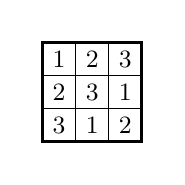
\begin{tikzpicture}[x=0.42cm,y=0.42cm]
\draw[line width=0.4pt] (1,0) -- (1,3);
\draw[line width=0.4pt] (0,1) -- (3,1);
\draw[line width=0.4pt] (2,0) -- (2,3);
\draw[line width=0.4pt] (0,2) -- (3,2);
\draw[line width=1pt] (0,0) rectangle (3,3);
\node at (0.5,2.5) {\small 1};
\node at (1.5,2.5) {\small 2};
\node at (2.5,2.5) {\small 3};
\node at (0.5,1.5) {\small 2};
\node at (1.5,1.5) {\small 3};
\node at (2.5,1.5) {\small 1};
\node at (0.5,0.5) {\small 3};
\node at (1.5,0.5) {\small 1};
\node at (2.5,0.5) {\small 2};
\path (-0.45,-0.45) rectangle (3.45,3.45);
\end{tikzpicture}\hspace{0.25cm}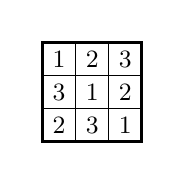
\begin{tikzpicture}[x=0.42cm,y=0.42cm]
\draw[line width=0.4pt] (1,0) -- (1,3);
\draw[line width=0.4pt] (0,1) -- (3,1);
\draw[line width=0.4pt] (2,0) -- (2,3);
\draw[line width=0.4pt] (0,2) -- (3,2);
\draw[line width=1pt] (0,0) rectangle (3,3);
\node at (0.5,2.5) {\small 1};
\node at (1.5,2.5) {\small 2};
\node at (2.5,2.5) {\small 3};
\node at (0.5,1.5) {\small 3};
\node at (1.5,1.5) {\small 1};
\node at (2.5,1.5) {\small 2};
\node at (0.5,0.5) {\small 2};
\node at (1.5,0.5) {\small 3};
\node at (2.5,0.5) {\small 1};
\path (-0.45,-0.45) rectangle (3.45,3.45);
\end{tikzpicture}\hspace{0.25cm}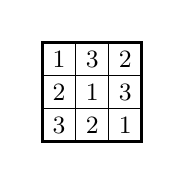
\begin{tikzpicture}[x=0.42cm,y=0.42cm]
\draw[line width=0.4pt] (1,0) -- (1,3);
\draw[line width=0.4pt] (0,1) -- (3,1);
\draw[line width=0.4pt] (2,0) -- (2,3);
\draw[line width=0.4pt] (0,2) -- (3,2);
\draw[line width=1pt] (0,0) rectangle (3,3);
\node at (0.5,2.5) {\small 1};
\node at (1.5,2.5) {\small 3};
\node at (2.5,2.5) {\small 2};
\node at (0.5,1.5) {\small 2};
\node at (1.5,1.5) {\small 1};
\node at (2.5,1.5) {\small 3};
\node at (0.5,0.5) {\small 3};
\node at (1.5,0.5) {\small 2};
\node at (2.5,0.5) {\small 1};
\path (-0.45,-0.45) rectangle (3.45,3.45);
\end{tikzpicture}\hspace{0.25cm}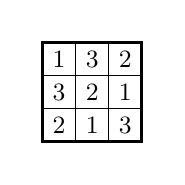
\begin{tikzpicture}[x=0.42cm,y=0.42cm]
\draw[line width=0.4pt] (1,0) -- (1,3);
\draw[line width=0.4pt] (0,1) -- (3,1);
\draw[line width=0.4pt] (2,0) -- (2,3);
\draw[line width=0.4pt] (0,2) -- (3,2);
\draw[line width=1pt] (0,0) rectangle (3,3);
\node at (0.5,2.5) {\small 1};
\node at (1.5,2.5) {\small 3};
\node at (2.5,2.5) {\small 2};
\node at (0.5,1.5) {\small 3};
\node at (1.5,1.5) {\small 2};
\node at (2.5,1.5) {\small 1};
\node at (0.5,0.5) {\small 2};
\node at (1.5,0.5) {\small 1};
\node at (2.5,0.5) {\small 3};
\path (-0.45,-0.45) rectangle (3.45,3.45);
\end{tikzpicture}\hspace{0.25cm}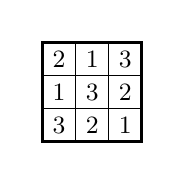
\begin{tikzpicture}[x=0.42cm,y=0.42cm]
\draw[line width=0.4pt] (1,0) -- (1,3);
\draw[line width=0.4pt] (0,1) -- (3,1);
\draw[line width=0.4pt] (2,0) -- (2,3);
\draw[line width=0.4pt] (0,2) -- (3,2);
\draw[line width=1pt] (0,0) rectangle (3,3);
\node at (0.5,2.5) {\small 2};
\node at (1.5,2.5) {\small 1};
\node at (2.5,2.5) {\small 3};
\node at (0.5,1.5) {\small 1};
\node at (1.5,1.5) {\small 3};
\node at (2.5,1.5) {\small 2};
\node at (0.5,0.5) {\small 3};
\node at (1.5,0.5) {\small 2};
\node at (2.5,0.5) {\small 1};
\path (-0.45,-0.45) rectangle (3.45,3.45);
\end{tikzpicture}\hspace{0.25cm}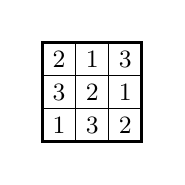
\begin{tikzpicture}[x=0.42cm,y=0.42cm]
\draw[line width=0.4pt] (1,0) -- (1,3);
\draw[line width=0.4pt] (0,1) -- (3,1);
\draw[line width=0.4pt] (2,0) -- (2,3);
\draw[line width=0.4pt] (0,2) -- (3,2);
\draw[line width=1pt] (0,0) rectangle (3,3);
\node at (0.5,2.5) {\small 2};
\node at (1.5,2.5) {\small 1};
\node at (2.5,2.5) {\small 3};
\node at (0.5,1.5) {\small 3};
\node at (1.5,1.5) {\small 2};
\node at (2.5,1.5) {\small 1};
\node at (0.5,0.5) {\small 1};
\node at (1.5,0.5) {\small 3};
\node at (2.5,0.5) {\small 2};
\path (-0.45,-0.45) rectangle (3.45,3.45);
\end{tikzpicture}}
\newcommand{\Mtwelveb}{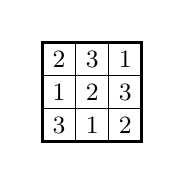
\begin{tikzpicture}[x=0.42cm,y=0.42cm]
\draw[line width=0.4pt] (1,0) -- (1,3);
\draw[line width=0.4pt] (0,1) -- (3,1);
\draw[line width=0.4pt] (2,0) -- (2,3);
\draw[line width=0.4pt] (0,2) -- (3,2);
\draw[line width=1pt] (0,0) rectangle (3,3);
\node at (0.5,2.5) {\small 2};
\node at (1.5,2.5) {\small 3};
\node at (2.5,2.5) {\small 1};
\node at (0.5,1.5) {\small 1};
\node at (1.5,1.5) {\small 2};
\node at (2.5,1.5) {\small 3};
\node at (0.5,0.5) {\small 3};
\node at (1.5,0.5) {\small 1};
\node at (2.5,0.5) {\small 2};
\path (-0.45,-0.45) rectangle (3.45,3.45);
\end{tikzpicture}\hspace{0.25cm}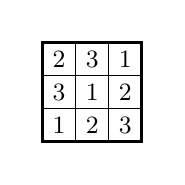
\begin{tikzpicture}[x=0.42cm,y=0.42cm]
\draw[line width=0.4pt] (1,0) -- (1,3);
\draw[line width=0.4pt] (0,1) -- (3,1);
\draw[line width=0.4pt] (2,0) -- (2,3);
\draw[line width=0.4pt] (0,2) -- (3,2);
\draw[line width=1pt] (0,0) rectangle (3,3);
\node at (0.5,2.5) {\small 2};
\node at (1.5,2.5) {\small 3};
\node at (2.5,2.5) {\small 1};
\node at (0.5,1.5) {\small 3};
\node at (1.5,1.5) {\small 1};
\node at (2.5,1.5) {\small 2};
\node at (0.5,0.5) {\small 1};
\node at (1.5,0.5) {\small 2};
\node at (2.5,0.5) {\small 3};
\path (-0.45,-0.45) rectangle (3.45,3.45);
\end{tikzpicture}\hspace{0.25cm}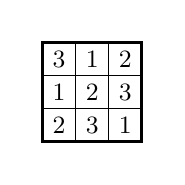
\begin{tikzpicture}[x=0.42cm,y=0.42cm]
\draw[line width=0.4pt] (1,0) -- (1,3);
\draw[line width=0.4pt] (0,1) -- (3,1);
\draw[line width=0.4pt] (2,0) -- (2,3);
\draw[line width=0.4pt] (0,2) -- (3,2);
\draw[line width=1pt] (0,0) rectangle (3,3);
\node at (0.5,2.5) {\small 3};
\node at (1.5,2.5) {\small 1};
\node at (2.5,2.5) {\small 2};
\node at (0.5,1.5) {\small 1};
\node at (1.5,1.5) {\small 2};
\node at (2.5,1.5) {\small 3};
\node at (0.5,0.5) {\small 2};
\node at (1.5,0.5) {\small 3};
\node at (2.5,0.5) {\small 1};
\path (-0.45,-0.45) rectangle (3.45,3.45);
\end{tikzpicture}\hspace{0.25cm}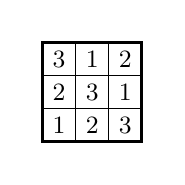
\begin{tikzpicture}[x=0.42cm,y=0.42cm]
\draw[line width=0.4pt] (1,0) -- (1,3);
\draw[line width=0.4pt] (0,1) -- (3,1);
\draw[line width=0.4pt] (2,0) -- (2,3);
\draw[line width=0.4pt] (0,2) -- (3,2);
\draw[line width=1pt] (0,0) rectangle (3,3);
\node at (0.5,2.5) {\small 3};
\node at (1.5,2.5) {\small 1};
\node at (2.5,2.5) {\small 2};
\node at (0.5,1.5) {\small 2};
\node at (1.5,1.5) {\small 3};
\node at (2.5,1.5) {\small 1};
\node at (0.5,0.5) {\small 1};
\node at (1.5,0.5) {\small 2};
\node at (2.5,0.5) {\small 3};
\path (-0.45,-0.45) rectangle (3.45,3.45);
\end{tikzpicture}\hspace{0.25cm}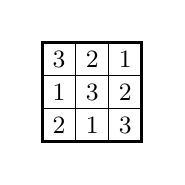
\begin{tikzpicture}[x=0.42cm,y=0.42cm]
\draw[line width=0.4pt] (1,0) -- (1,3);
\draw[line width=0.4pt] (0,1) -- (3,1);
\draw[line width=0.4pt] (2,0) -- (2,3);
\draw[line width=0.4pt] (0,2) -- (3,2);
\draw[line width=1pt] (0,0) rectangle (3,3);
\node at (0.5,2.5) {\small 3};
\node at (1.5,2.5) {\small 2};
\node at (2.5,2.5) {\small 1};
\node at (0.5,1.5) {\small 1};
\node at (1.5,1.5) {\small 3};
\node at (2.5,1.5) {\small 2};
\node at (0.5,0.5) {\small 2};
\node at (1.5,0.5) {\small 1};
\node at (2.5,0.5) {\small 3};
\path (-0.45,-0.45) rectangle (3.45,3.45);
\end{tikzpicture}\hspace{0.25cm}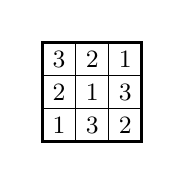
\begin{tikzpicture}[x=0.42cm,y=0.42cm]
\draw[line width=0.4pt] (1,0) -- (1,3);
\draw[line width=0.4pt] (0,1) -- (3,1);
\draw[line width=0.4pt] (2,0) -- (2,3);
\draw[line width=0.4pt] (0,2) -- (3,2);
\draw[line width=1pt] (0,0) rectangle (3,3);
\node at (0.5,2.5) {\small 3};
\node at (1.5,2.5) {\small 2};
\node at (2.5,2.5) {\small 1};
\node at (0.5,1.5) {\small 2};
\node at (1.5,1.5) {\small 1};
\node at (2.5,1.5) {\small 3};
\node at (0.5,0.5) {\small 1};
\node at (1.5,0.5) {\small 3};
\node at (2.5,0.5) {\small 2};
\path (-0.45,-0.45) rectangle (3.45,3.45);
\end{tikzpicture}}


\renewcommand{\arraystretch}{1.15}
\renewcommand{\normalsize}{\fontsize{10.5}{13.2}\selectfont}

\begin{document}
\RaggedRight

{\color{mute}\small Student packets: K--1 (F05-K-v4, 7 pages), 2--3 (F05-M-v4, 9 pages), 4--5 (F05-U-v4, 8 pages). Every answer here was recomputed by guide-src/check.py from the student pages.}

\section{1. The idea of the week}

Stand towers of different heights in a row, put your eye down at the table about a foot from one end, and look along the row. You see a tower when it is taller than every tower in front of it; a tower with a taller one in front of it is hidden. The tallest tower is seen from both ends. So you see just 1 tower from an end exactly when the tallest tower stands at that end, and no row of two or more towers shows 1 from both ends.

A \emph{city} is a square grid with one tower on each square and each height once in every row and every column. The numbers around the edge say how many towers are seen along each row and column from that side. Some sets of edge numbers fit exactly one city, some fit several and some fit none. The children build, look, and then reason about which rows and cities are possible.

\begin{tabularx}{\linewidth}{@{}>{\bfseries}p{2.3cm}X@{}}
\toprule
Table & A good session looks like this \\
\midrule
K--1 & Every child builds rows of three towers, gets down to table level and counts from both ends, and helps find the six different rows. The pairs play several rounds of the hidden-row game (Problem 4). Someone says why no row shows 1 and 1. \\
Grades 2--3 & Each child builds a city and writes its twelve numbers, then solves two or three puzzles. At least one pair makes a puzzle for the other pair. Someone notices that the tallest tower is always seen, or that every city's numbers add to 22. \\
Grades 4--5 & The children climb the ladder of puzzles (fewer numbers each time), find the four cities of Problem 4, and make a puzzle with few numbers for a partner. Someone makes a claim (fewest numbers, or a pattern in the Problem 7 table) and tests it. \\
\bottomrule
\end{tabularx}

\section{2. Materials and preparation}

\textbf{Snap cubes} (3/4 inch). Pre-build every tower before the session and put each child's set in its own bag or cup. This saves a lot of time: a 4--5 child's set is sixteen towers, and children can start building rows at once.

\begin{tabularx}{\linewidth}{@{}>{\bfseries}l X l r r r@{}}
\toprule
Table & Each child gets & Towers to pre-build & In use & Spare & Total \\
\midrule
K--1 (4) & 6 cubes: one tower each of 1, 2, 3 & 12 (4 of each height) & 24 & 6 & 30 \\
2--3 (4) & 18 cubes: three towers each of 1, 2, 3 & 36 (12 of each height) & 72 & 10 & 82 \\
4--5 (3) & 40 cubes: four towers each of 1, 2, 3, 4 & 48 (12 of each height) & 120 & 10 & 130 \\
\midrule
All & & 96 towers & 216 & 26 & 242 \\
\bottomrule
\end{tabularx}

The launch borrows one K--1 set. In K--1 Problems 5--7 each pair pools its two sets and snaps a 1-tower onto a 3-tower to make a 4 (10 of the pair's 12 cubes). If colours allow, make all towers of one height the same colour at the 2--3 and 4--5 tables; a city is then right when no colour repeats in a row or column.

\textbf{Also:} file folders as screens, stood open in a V: 2 at K--1 (one per pair), 4 at 2--3, 3 at 4--5, and 1 for the launch (10). Pencils, a small whiteboard per child, scrap paper. A few sheets of plain paper per table: laid lengthwise off the end of a row, the long side (11 inches) marks ``about a foot'' for the eye. Leave a foot of clear table beyond the end of every row. Nothing needs cutting or taping.

\textbf{Printing} (single-sided, US Letter, 100\%). Hand out one page at a time and keep the next page in your hand.

\begin{xltabular}{\linewidth}{@{}>{\bfseries}l p{5.4cm} X@{}}
\toprule
Table & Print & Notes \\
\midrule
\endhead
K--1 & k-1.pdf, pages 1--7: 5 of each & One per child and one for you. Read each problem aloud. \\
2--3 & grades-2-3.pdf, pages 1--9: 5 of each, plus 4 more of page 7 & The large grids on pages 2--7 have 1-inch squares, so cubes stand on them. Page 7 is two blank grids, spare for Problem 5 puzzles. \\
4--5 & grades-4-5.pdf, pages 1--8: 4 of each, plus 6 more of page 2 & Only page 2 has a 1-inch 4-by-4 grid. The grids on pages 3--8 have squares of 1.7\,cm or less, smaller than a cube, so to build a puzzle a child copies its numbers onto a page-2 copy. In Problem 5 the hidden city is built on one. \\
\bottomrule
\end{xltabular}

\textbf{Test with the real cubes the evening before.}
\begin{enumerate}
\item Stand towers 3, 1, 2, 4 on a 1-inch grid. With your chin on the table a foot from the 3, you see 2 towers (the 3 and the 4). Closer than about 9 inches the 4 hides behind the 3 and the count comes out wrong. At a foot, every row of three or four gives the right count.
\item Build a 3-by-3 city and look along its middle row from table level. If the neighbouring rows get in the way, show children how to slide that row out toward them without changing its order, look, and slide it back. Edge rows can be checked in place.
\item A cube fits inside a 1-inch square, a 4-cube tower stands without tipping, and a folder stood open hides a 4-cube tower (3 inches).
\end{enumerate}

\section{3. The hour}

\begin{tabularx}{\linewidth}{@{}>{\bfseries}l X@{}}
\toprule
0:00--0:05 & Running around. \\
0:05--0:08 & Whole-group launch at one table (below). \\
0:08--0:48 & Work at the three tables in pairs. Switch to the fallback when attention runs out. \\
0:48--0:55 & Sharing question, all together. Then cubes back into their bags. \\
\bottomrule
\end{tabularx}

\textbf{Launch (2--3 minutes, organizer).} Set out towers of 1, 2 and 3 cubes, with a sheet of paper laid lengthwise at each end of the row. Children stand round the table.
\begin{enumerate}
\item Stand the row 2, 1, 3. Say: ``Each tower stands in the row once. Put your chin on the table at the end of this paper and look along the row. You see a tower when it is taller than every tower in front of it.''
\item One child puts a chin down at the left end. Ask: ``How many towers do you see?'' (2: the 2 and the 3; the 1 hides behind the 2.) A second child looks from the right end: 1 (the 3 hides the others).
\item The move: ``Change the row so that you see 3 towers from this end.'' One child moves the towers (to 1, 2, 3 from that end). Another child checks with a chin on the table. Ask what the other end shows now (1).
\item Hold up a folder: ``Sometimes one of you hides a row behind this and says the two numbers. Your partner builds a row that shows them.'' Send children to their tables.
\end{enumerate}

\begin{xltabular}{\linewidth}{@{}>{\bfseries}p{1.25cm}X X@{}}
\toprule
Table & Pairs & Fallback when attention runs out \\
\midrule
\endhead
K--1 & Two pairs, each a kindergartner with a first grader. One builds, the other gets down and counts; swap at each new row. You read each problem aloud and point at the picture. & You hide a row of three behind the folder and say the two numbers. Each child builds a row that shows them and checks it at table level. Lift the folder: any row that shows the numbers is right, even if it is not yours. \\
2--3 & Two pairs. One builds, the other checks every edge number by eye; swap at each city or puzzle. & Hidden row of four: the hider builds a row of 1, 2, 3, 4 cubes behind the folder (a 4 from the spares), checks it, and says the two numbers; the partner builds a row that fits. \\
4--5 & One pair works; the third child is referee, checking views by eye and each height once per row and column, and hunting for a second city in Problems 4--6. Rotate the referee at each new problem. & Fewest questions: one child builds a 3-by-3 city behind the folder. The partner asks for one edge number at a time (``left of the top row?'') until they can build the city. Fewest numbers asked wins; two can be enough. \\
\bottomrule
\end{xltabular}

\textbf{Sharing question (all tables):} ``Can a row ever show just 1 tower from both ends? Why not?'' Every table meets this (K--1 Problem 3, 2--3 Problem 1, 4--5 Problem 1). The answer a child can give: to see only 1 from an end, the tallest tower must stand at that end, and there is only one tallest tower.

\section{4. Table by table}

\textbf{How answers are written.} A row is written by its heights from left to right: 132 is a 1-cube tower, then a 3-cube tower, then a 2-cube tower. ``2 and 1'' or (2,1) means 2 seen from the left end and 1 from the right end. In a city, row 1 is the top row and column 1 the left column; ``above column 2'' is the edge place over column 2. Small solved grids show the puzzle's edge numbers in grey. \core{} problems are for everyone; \further{} problems are for children who get there. Hints are in the order to give them.

\tsub{K--1 (parent volunteer)}

Page 1 picture (row 1\,3\,2, eye on the left): you see 2 towers, the 1 and the 3; the 2 hides behind the 3.

\textbf{Things to say:} ``Chin on the table at the end of the paper.'' ``Point to each tower top you can see.'' ``Is a tower hiding behind a taller one?'' ``Which tower can you always see?'' ``How do you know there are no more?''

\pb{1}{\core}{Build the two pictured rows and write in each circle how many towers you see from that end.}
\begin{pbody}
\item[Answer] Left picture \tw{1,3,2}\ 1\,3\,2: 2 and 2. Right picture \tw{3,2,1}\ 3\,2\,1: 1 and 3.
\item[Hints] \hint1 ``Chin down. Point to each top you can see.'' \hint2 ``Which tower is in front of the 2? Is it taller?'' \hint3 Walk a finger along the row from that end; count a tower each time it is taller than all before it.
\end{pbody}

\pb{2}{\core}{Find every way to stand the three towers in a row, and draw each with its two numbers. There are eight frames; two stay empty.}
\begin{pbody}
\item[Answer] Six rows: \\[2pt]
\begin{tabular}{@{}l@{\quad}l@{\qquad}l@{\quad}l@{\qquad}l@{\quad}l@{}}
\tw{1,2,3} & 123: 3 and 1 & \tw{2,1,3} & 213: 2 and 1 & \tw{3,1,2} & 312: 1 and 2 \\
\tw{1,3,2} & 132: 2 and 2 & \tw{2,3,1} & 231: 2 and 2 & \tw{3,2,1} & 321: 1 and 3 \\
\end{tabular}
\item[Why all] The 3 can stand first, in the middle, or last. Each time, the other two can swap. 2 + 2 + 2 = 6.
\item[Hints] \hint1 ``Put the 3 at the left end. How many ways can the other two stand?'' \hint2 ``Now put the 3 in the middle. Then at the right end.'' \hint3 ``Is this row the same as one you drew already?''
\lastitem[If stuck] Stop after three or four rows and go to Problem 4.
\end{pbody}

\pb{3}{\core}{Build a row for each card, or put an X on it.}
\begin{pbody}
\item[Answer] \begin{tabular}[t]{@{}l l@{\qquad}l l@{\qquad}l l@{}}
1 and 3 & 321 & 3 and 3 & X & 1 and 1 & X \\
2 and 1 & 213 & 2 and 2 & 132 or 231 & 1 and 2 & 312 \\
\end{tabular}
\item[Why X] 3 and 3: ``To see all 3 from the left, the row must go short, middle, tall. Then from the right you see only the tall one.'' 1 and 1: ``To see only 1 from the left, the tall tower must be at the left end. To see only 1 from the right, it must be at the right end. There is only one tall tower.''
\item[Hints] \hint1 ``Which tower can you always see from both ends?'' \hint2 ``To see just 1 from this end, where must the tall tower go?'' \hint3 For an X card: ``Try to build it. What goes wrong?''
\lastitem[If stuck] Do the 1-and-3, 2-and-1 and 2-and-2 cards only.
\end{pbody}

\pb{4}{\core}{The hidden-row game. This is the main activity at this table; play it for as long as it holds them.}
\begin{pbody}
\item[Answer] The numbers a hider can say: 1 and 2, 1 and 3, 2 and 1, 2 and 2, 3 and 1. If a hider says 1 and 1, 3 and 3, 2 and 3, or 3 and 2, they miscounted: lift the folder and count together. Any row that shows the numbers is right; for 2 and 2 there are two rows, 132 and 231. The pictured hidden row is 231 (2 and 2). After each round, lift the folder and both children check both rows at table level.
\item[Hints] \hint1 ``Where does the tall tower go for these numbers?'' \hint2 ``Find the card in Problem 3 with these numbers.''
\end{pbody}

\pb{5}{\further}{With towers of 1, 2, 3, 4: every row that shows just 1 from the left.}
\begin{pbody}
\item[Answer] 4123, 4132, 4213, 4231, 4312, 4321. Eight frames; two stay empty.
\item[Why all] ``If any tower stands in front of the 4, you see it and the 4. So the 4 is first, and the other three stand behind it in the six ways from Problem 2.''
\item[Hints] \hint1 ``Where must the 4 stand so it hides all the others?'' \hint2 ``Now look at your Problem 2 page.''
\end{pbody}

\pb{6}{\further}{Every row of four that shows 2 from each end.}
\begin{pbody}
\item[Answer] With the 4 second: 1423, 2413, 3412. With the 4 third: 2143, 3142, 3241. Six rows; eight frames.
\item[Why all] The 4 cannot be at an end, or that end sees only 1. With the 4 second, the last two towers go short then tall, so the right end sees the last one and the 4; the first tower can be 1, 2 or 3. With the 4 third, it is the same turned around.
\item[Hints] \hint1 ``Can the 4 stand at an end?'' \hint2 ``Put the 4 second. Which way round must the last two go?'' \hint3 ``Now put the 4 third.''
\end{pbody}

\pb{7}{\further}{Build a row of four for each card, or put an X on it.}
\begin{pbody}
\item[Answer] \begin{tabular}[t]{@{}l l@{\qquad}l l@{}}
2 and 3 & 1432, 2431 or 3421 & 3 and 1 & 1324, 2134 or 2314 \\
1 and 4 & 4321 & 4 and 2 & X \\
3 and 3 & X & 1 and 2 & 4123 or 4213 \\
\end{tabular}
\item[Why X] 3 and 3: ``You see the 4 from both ends. To see 3 from the left you need 2 towers left of the 4, and to see 3 from the right 2 more on its right. That is 5 towers; we have 4.'' 4 and 2: ``To see all 4 from the left the row must be 1234, and then the right end sees only the 4.''
\end{pbody}

\tsub{Grades 2--3 (mathematician)}

\pb{1}{\core}{All orders of 1, 2, 3 with their views; which pairs never occur, and why.}
\begin{pbody}
\item[Answer] 123 (3,1), 132 (2,2), 213 (2,1), 231 (2,2), 312 (1,2), 321 (1,3). Never: (1,1), (3,3), (2,3), (3,2). Eight slots; two spare.
\item[Why] The 3 is seen from both ends. Seeing 1 from an end puts the 3 at that end, and it cannot be at both. Seeing 3 from an end forces 1, 2, 3 from that end, and then the other end sees only the 3.
\item[Hints] \hint1 ``Put the 3 first. How many rows now?'' \hint2 ``Which tower do you see from both ends?'' \hint3 ``If you see 3 from the left, what must the row be?''
\lastitem[If stuck] Skip the ``explain why'' and go on to building a city in Problem 2.
\end{pbody}

\pb{2}{\core}{Build two different cities and write their edge numbers.}
\begin{pbody}
\item[Answer] \begin{tabular}[t]{@{}m{11.6cm}@{\hspace{0.4cm}}m{2.2cm}@{}}
Any of the 12 cities; each uses all 18 cubes. The twelve edge numbers of a 3-by-3 city always add to 22 (Problem 7), so any other total means a miscount. An example with its numbers is on the right. & \Msample
\end{tabular}
\item[Hints] \hint1 ``Build the top row 1, 2, 3. Which heights can stand under the 1?'' \hint2 ``Make the next row by sliding the top row one place along.'' \hint3 For a middle row: slide it out to look, then put it back.
\end{pbody}

\pb{3}{\core}{Four puzzles (pages 3--4). Puzzle 3 has no city.}
\begin{pbody}
\item[Answer] Solutions, with each puzzle's numbers in grey:\\[2pt]
\begin{tabular}{@{}c@{\hspace{0.5cm}}c@{\hspace{0.5cm}}c@{\hspace{0.5cm}}c@{}}
\MthreeSola & \MthreeSolb & \raisebox{0.95cm}{\parbox{2.2cm}{\centering no city}} & \MthreeSold \\
puzzle 1 & puzzle 2 & puzzle 3 & puzzle 4
\end{tabular}
\item[Starts] Puzzle 1: the 1 above column 2 puts a 3 at its top; the 1 right of row 3 puts a 3 at its right end; the 3 above column 3 makes column 3 read 1, 2, 3 down. Puzzle 2: the 1 left of row 2 puts a 3 at its left end. Puzzle 4: only a 1 can stand at the bottom of column 2 (row 3 needs a 3 or a 1 in its middle; column 2 needs a 1 or a 2 at its bottom).
\item[Why not] Puzzle 3 (2, 2, 2 above): the 3 in the top row stands at the top of some column. Looking down that column you see only the 3, so its number would be 1, not 2.
\item[Hints] \hint1 ``Find a 1 on the edge. Where must the 3 stand?'' \hint2 ``Find a 3 on the edge. What must that line be?'' \hint3 ``Build it on the grid and check each number by eye.''
\lastitem[If stuck] Skip puzzle 3, or keep it for last as a ``why not'' question.
\end{pbody}

\pb{4}{\core}{Find every city for the 1 above column 1 and the 2 left of row 3; then add one number.}
\begin{pbody}
\item[Answer] Three cities: \raisebox{-0.45\height}{\MfourSola}\ A \quad \raisebox{-0.45\height}{\MfourSolb}\ B \quad \raisebox{-0.45\height}{\MfourSolc}\ C \\[2pt]
One added number that leaves only A: 3 above column 2, 3 left of row 2, or 2 right of row 1. Only B: 3 above column 3, 2 below column 2, 1 below column 3, 2 right of row 2, or 1 right of row 3. Only C: 3 below column 1.
\item[Hints] \hint1 ``The 1 above column 1: where is the 3 in that column?'' \hint2 ``Row 1 starts with 3. How can it go on?'' \hint3 ``Lay two of your cities side by side. Which edge number is different?''
\end{pbody}

\pb{5}{\further}{Hidden city for a partner; fewest numbers, and why fewer cannot work.}
\begin{pbody}
\item[Answer] Fewest: 2. One number is never enough: if it looks along column 1, swap columns 2 and 3. That is still a city, the number does not change, and the city is different (the same for any line). With cubes: slide the two other columns past each other. Two can be enough: 3 left of row 1 and 3 above column 1 fit only 123/231/312, and so does puzzle 4 of Problem 3. (156 two-number puzzles fit exactly one city.)
\item[Hints] \hint1 ``Your partner found a second city. Which number would rule it out?'' \hint2 ``With one number above column 1, swap columns 2 and 3. Does the number change?'' \hint3 ``Try two 3s that meet at a corner.''
\end{pbody}

\pb{6}{\further}{How many 3-by-3 cities, and why the list is complete.}
\begin{pbody}
\item[Answer] \begin{tabular}[t]{@{}l@{}}12, in the order of their top rows:\\[3pt]\Mtwelvea\\[2pt]\Mtwelveb\end{tabular}
\item[Why all] The top row is one of the 6 orders. The second row must put a new height in every column, which leaves exactly two choices: the top row shifted one place left or one place right, wrapping round. The third row is then forced. 6 $\times$ 2 = 12.
\item[Hints] \hint1 ``Keep the top row 123. How many cities start that way?'' \hint2 ``Now use each of your six rows from Problem 1 as the top row.''
\end{pbody}

\pb{7}{\further}{Which totals of the twelve edge numbers are possible.}
\begin{pbody}
\item[Answer] Only 22.
\item[Why] A row's two numbers add to 4, except when its 1 is in the middle (213, 312): then they add to 3. Each column holds one 1, so exactly one row has its 1 in the middle; in the same way exactly one column does. Total: 6 $\times$ 4 $-$ 2 = 22.
\item[Hints] \hint1 ``Add up the numbers of the cities you already wrote.'' \hint2 ``For one row, when do its two numbers add to 3, and when to 4?'' \hint3 ``Where can the 1s be?''
\end{pbody}

\tsub{Grades 4--5 (organizer)}

\pb{1}{\core}{Rows of 1, 2, 3, 4 for eight cards.}
\begin{pbody}
\item[Answer] \begin{tabular}[t]{@{}l l@{\qquad}l l@{}}
(1,2) & 4123, 4213 & (1,4) & 4321 \\
(2,3) & 1432, 2431, 3421 & (1,1) & impossible \\
(3,3) & impossible & (3,2) & 1243, 1342, 2341 \\
(2,2) & 1423, 2143, 2413, 3142, 3241, 3412 & (4,2) & impossible \\
\end{tabular}
\item[Why] If the 4 is in place $j$, the towers seen from the left are in places 1 to $j$ and those seen from the right in places $j$ to 4, so $L\le j$, $R\le 5-j$ and $L+R\le 5$. This rules out (3,3) and (4,2); (1,1) needs the 4 at both ends. With cubes: ``the 4 is seen from both ends; 3 and 3 needs two towers on each side of it.''
\item[Hints] \hint1 ``Where is the 4 when you see 1 from the left?'' \hint2 ``Count the towers on each side of the 4.''
\end{pbody}

\pb{2}{\core}{Build one 4-by-4 city and write its sixteen numbers.}
\begin{pbody}
\item[Answer] Any of the 576 cities; each uses all 40 cubes. Inner rows: slide out to look.
\item[Hints] \hint1 ``Start with row 1 as 1234. What can row 2 be?'' \hint2 ``Check each column as you add a row.''
\end{pbody}

\pb{3}{\core}{The ladder: six puzzles with 12, 8, 6, 6, 5 and 4 numbers (pages 3--4, read left to right).}
\begin{pbody}
\item[Answer] Solutions, with each puzzle's numbers in grey:\\[2pt]
\begin{tabular}{@{}c@{\hspace{0.15cm}}c@{\hspace{0.15cm}}c@{\hspace{0.15cm}}c@{\hspace{0.15cm}}c@{\hspace{0.15cm}}c@{}}
\UthreeSola & \UthreeSolb & \UthreeSolc & \UthreeSold & \UthreeSole & \UthreeSolf \\
A & B & C & D & E & F
\end{tabular}
\item[Starts] A: the 4 above column 1 makes it read 1, 2, 3, 4 down; the 1s above column 3 and left of row 4 place two 4s. B: the 4 below column 3 makes it read 4, 3, 2, 1 down; the 1s left of row 2 and right of row 4 place two 4s. C: the 1 right of row 4 places a 4; column 2 shows 2 from the top and 3 from the bottom, so its 4 is in row 2 (the (2,3) card of Problem 1). D: the 4 above column 3 makes it read 1, 2, 3, 4 down; the 1 left of row 2 places a 4. E has no 1s or 4s and F has only 2s: start by marking where each 4 can stand.
\item[Note] A--C fall to two passes of one-line-at-a-time reasoning, D to three; E and F need five and seven passes, and a child may need to try a case and build it.
\item[Hints] \hint1 ``Find a 1 or a 4 on the edge. What does it tell you?'' \hint2 ``Next to a 3, the 4 is in the third or fourth square; next to a 2, it is not in the first. Where can each 4 go?'' \hint3 ``Copy the numbers onto a page-2 grid and build it.''
\lastitem[If stuck] Do A and B with cubes on page-2 grids, then go to Problem 4.
\end{pbody}

\pb{4}{\core}{Every city with a 4 above column 1 and a 4 left of row 1; then add one number.}
\begin{pbody}
\item[Answer] Four cities: \raisebox{-0.45\height}{\UfourSola}\ A \quad \raisebox{-0.45\height}{\UfourSolb}\ B \quad \raisebox{-0.45\height}{\UfourSolc}\ C \quad \raisebox{-0.45\height}{\UfourSold}\ D \\[2pt]
Only B: 3 below column 3, 3 below column 4, 3 right of row 3, or 3 right of row 4. Only C: 3 above column 2, 3 left of row 2, 2 below column 4, or 2 right of row 4. A and D cannot be singled out: they have the same sixteen numbers (this answers Problem 9). Each of the eight answers is a three-number puzzle with one city, the fewest possible (Problem 5).
\item[Hints] \hint1 ``What do the two 4s say about row 1 and column 1?'' \hint2 ``Row 2 starts with 2. What can come next?'' \hint3 ``Lay two of your cities side by side. Which edge numbers differ?''
\end{pbody}

\pb{5}{\further}{Hidden city for a partner with as few numbers as possible.}
\begin{pbody}
\item[Answer] Fewest: 3. No two-number 4-by-4 puzzle fits exactly one city (computer check over all 576 cities); 1600 three-number puzzles do. If both numbers look along rows, at least two other rows are untouched and can be swapped; the same for columns. The row-and-column case has no short argument here. The solver hunts for a second city; the referee settles it by building.
\item[Hints] \hint1 ``Problem 4 had two numbers and four cities. Add one number.'' \hint2 ``Your partner found a second city. Which edge number differs between the two?''
\end{pbody}

\pb{6}{\further}{Three numbers, none a 4, exactly one city.}
\begin{pbody}
\item[Answer] \begin{tabular}[t]{@{}m{11.3cm}@{\hspace{0.4cm}}m{2.6cm}@{}}
Possible: 40 such puzzles, 16 of them all 3s. Example (right): 3 above column 1, 3 above column 3 and 3 left of row 4. Another: 3 below column 3 and 3 left of rows 1 and 4, with city 1243/3421/4132/2314. & \UsixSol
\end{tabular}
\item[Hints] \hint1 ``Next to a 3, where can the 4 be?'' \hint2 ``Place three 3s so that together they pin down the 4s.''
\end{pbody}

\pb{7}{\further}{Sort the 24 rows of four by their two views.}
\begin{pbody}
\item[Answer] \begin{tabular}[t]{@{}c|cccc|c@{}}
L\,$\backslash$\,R & 1 & 2 & 3 & 4 & total \\ \hline
1 & 0 & 2 & 3 & 1 & 6 \\
2 & 2 & 6 & 3 & 0 & 11 \\
3 & 3 & 3 & 0 & 0 & 6 \\
4 & 1 & 0 & 0 & 0 & 1 \\
\end{tabular}
\quad\parbox[t]{8.3cm}{Symmetric, because turning a row round swaps its two numbers. Zero wherever $L+R$ is more than 5, and at (1,1). Row totals 6, 11, 6, 1.}
\item[Hints] \hint1 ``Your Problem 1 cards already fill eight cells.'' \hint2 ``Turn a row round. What happens to its two numbers?'' \hint3 ``Where is the 4 in the rows with 1 from the left?''
\end{pbody}

\pb{8}{\further}{Rows of five: how many show exactly 1, and exactly 2, from the left.}
\begin{pbody}
\item[Answer] 24 and 50.
\item[Why] Exactly 1: the 5 is first and the other four follow in $4\times3\times2\times1 = 24$ orders. Exactly 2, by the first tower $h$: the 5 must come before every other tower taller than $h$. First tower 4: all 24 orders of the rest; 3: half of them (5 before 4), 12; 2: a third, 8; 1: a quarter, 6. Total 50. Or from Problem 7: put the 1-tower into a row of 2, 3, 4, 5. In front it adds a seen tower; in any of the other 4 places it is hidden. So $6 + 4\times 11 = 50$.
\item[Hints] \hint1 ``Where must the 5 be to see only 1?'' \hint2 ``If the first tower is a 4, where can the 5 go?''
\end{pbody}

\pb{9}{\further}{Can two cities share all sixteen numbers?}
\begin{pbody}
\item[Answer] \begin{tabular}[t]{@{}m{2.6cm}@{\hspace{0.2cm}}m{2.6cm}@{\hspace{0.4cm}}m{8.6cm}@{}}
\UnineA & \UnineB & Yes, for example these two, which are cities A and D of Problem 4. They differ only in the middle 2-by-2 block.
\end{tabular}\\[1pt] In rows 2 and 3 and columns 2 and 3 the middle 1 is hidden and the middle 4 is seen either way, so no edge number changes. In all, 66 sets of sixteen numbers belong to two or more cities (204 of the 576 cities). No two 3-by-3 cities share their numbers.
\item[Hints] \hint1 ``In Problem 4, could you single out every city by adding one number?'' \hint2 ``Swap a 2-by-2 block in the middle of a city. Does any edge number change?''
\end{pbody}

\section{5. The mathematics behind the week}

\textbf{Seen towers are records.} A row is a permutation $p$ of $1,\dots,n$, and the towers seen from the left are its left-to-right maxima. The tallest tower is a record from both ends; $L=1$ exactly when $n$ is first. If $n$ is in place $j$, every tower seen from the left is in places $1..j$ and every one seen from the right in places $j..n$, so $L+R\le n+1$, with equality exactly when the row rises to $n$ and then falls ($2^{n-1}$ rows).

\textbf{Counting by the number seen.} Let $c(n,k)$ be the number of rows with $k$ seen from the left. Insert the shortest tower into a row of $2,\dots,n$: in front it is one more record, and in any of the other $n-1$ places it is hidden and hides nothing. So $c(n,k)=c(n-1,k-1)+(n-1)\,c(n-1,k)$: these are the unsigned Stirling numbers of the first kind, with $\sum_k c(n,k)x^k = x(x+1)\cdots(x+n-1)$. Rows: $n=3$: 2, 3, 1; $n=4$: 6, 11, 6, 1; $n=5$: 24, 50, 35, 10, 1. The tower in place $j$ is a record with probability $1/j$, so on average $1+\frac12+\dots+\frac1n\approx\ln n$ towers are seen. Cutting a row before each record gives one cycle per record (Foata's bijection), so the same numbers count permutations by cycles.

\textbf{Both ends.} The number of rows with views $(a,b)$ is $\binom{a+b-2}{a-1}\,c(n-1,a+b-2)$. Remove $n$. Cut the part left of $n$ before each of its left-to-right records, and the part right of $n$ after each of its right-to-left records. This gives $a+b-2$ blocks, each led (on the left) or ended (on the right) by its largest element, so each block is a cycle; on the left the blocks appear in increasing order of their maxima and on the right in decreasing order. Conversely, pick a permutation of $1..n-1$ with $a+b-2$ cycles and choose which $a-1$ of them go left. For $n=4$, $(2,2)$ gives $\binom21 c(3,2)=6$, as in 4--5 Problem 7.

\textbf{Cities} are Latin squares: 2, 12 and 576 of orders 2, 3 and 4 (and 161\,280 of order 5). For order 3 the twelve edge numbers always total 22 (2--3 Problem 7), and the twelve cities have twelve different sets of edge numbers. The fewest numbers that fix a city is 2 for order 3 (one number: swap the two lines parallel to it that it does not see) and 3 for order 4 (by computer). In order 4, edge numbers do not always fix the city: 66 sets are shared by two or more cities. Of the 262 such pairs, 152 differ by switching a 2-by-2 block $\begin{smallmatrix}a&b\\b&a\end{smallmatrix}$ that no view can detect.

\textbf{Where it goes.} Records in random permutations and the secretary problem; Stirling numbers and cycles; Skyscrapers puzzles at 5-by-5 and 6-by-6; counting Latin squares; and smallest critical sets, of which ``fewest numbers'' is a small case (for Sudoku the answer is 17 clues).

\newpage
\section{6. What to write down after the session}

Fill in one block per table the same evening. For each claim, tick how far it got: \emph{tried} (built or drew some cases), \emph{guessed} (said it without testing), \emph{checked in some cases}, \emph{explained} (gave a reason that covers every case). Claims to listen for: ``the tallest is always seen'', ``1 and 1 is impossible'', ``there are six rows of three'', ``every city adds to 22'', ``one number is never enough'', ``two cities can have the same numbers''.

\newcommand{\recblock}[2]{%
\noindent\textbf{#1}\quad Problems reached (circle):\enspace #2\par\vspace{2pt}
\noindent\begin{tabularx}{\linewidth}{@{}|X|@{}}
\hline
\small What children tried and said:\\[1.25cm]
\hline
\small A drawing or claim worth keeping (copy it, with the child's words):\\[1.05cm]
\hline
\end{tabularx}\par\vspace{2pt}
\noindent\begin{tabularx}{\linewidth}{@{}|X|c|c|>{\centering\arraybackslash}p{2.1cm}|c|@{}}
\hline
\small Claim & \small tried & \small guessed & \small checked in some cases & \small explained \\
\hline
 & & & & \\[0.2cm] \hline
 & & & & \\[0.2cm] \hline
\end{tabularx}\par\vspace{6pt}}

\recblock{K--1}{1\enspace 2\enspace 3\enspace 4 (rounds played: \rule{1cm}{0.4pt})\enspace 5\enspace 6\enspace 7}
\recblock{Grades 2--3}{1\enspace 2\enspace 3 (puzzles: 1 2 3 4)\enspace 4\enspace 5\enspace 6\enspace 7}
\recblock{Grades 4--5}{1\enspace 2\enspace 3 (A B C D E F)\enspace 4\enspace 5\enspace 6\enspace 7\enspace 8\enspace 9}


\end{document}
